\documentclass{ximera}

\input{../preamble.tex}
\outcome{Convert between polar and Cartesian coordinates.}
\outcome{Convert between the Cartesian and polar reprentation of a curve.}
\outcome{Determine whether different polar representations represent the same point in the $(x,y)$-plane} 
\outcome{Use the Cartesian to polar method to plot polar graphs.}
\outcome{Understand the difference between a curve and the choice of coordinates used to describe the curve}

\title[Dig-In:]{Introduction to polar coordinates}

\begin{document}
\begin{abstract}
Polar coordinates are coordinates based on an angle and a radius.
\end{abstract}
\maketitle

\section{Polar coordinates}

%Now we focus on a special type of parametric equations, those of the
%form:
%\begin{align*} 
%  x(\theta) &= r(\theta) \cdot \cos(\theta)\\
%  y(\theta) &= r(\theta) \cdot \sin(\theta)
%\end{align*}
%where $r(\theta)$ is a function of $\theta$.  When working with
%parametric equations of this form, it is common to notate
%\[
%(r \cdot \cos(\theta), r\cdot \sin(\theta)) \text{ as } (r,\theta)
%\]
%and state that we are working in \textit{polar coordinates}.

\begin{definition}
  An ordered pair consisting of a radius and an angle $(r,\theta)$
  can be graphed as
  \begin{align*}
    x &= r\cdot \cos(\theta)\\
    y &= r\cdot \sin(\theta)
  \end{align*}
  meaning:
  \begin{image}[2in]
    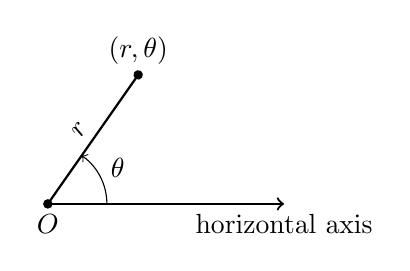
\begin{tikzpicture}
	\draw[thick,->] (0,0) node [below] {$O$} -- (3,0) node [below] {horizontal axis} ;
	\filldraw (0,0) circle (1.5pt);
	\filldraw [rotate=55] (2,0) circle (1.5pt);
	\draw [thick,rotate=55] (0,0)-- node [rotate=55,pos=.5,above] {$r$} (2,0) node [above] {$(r,\theta)$};
	\draw [->] (.75,0) arc(0:55:.75); 
	\draw [rotate=27.5] (1,0) node {$\theta$};
    \end{tikzpicture}
  \end{image}
  Coordinates of this type are called \dfn{polar coordinates}.
\end{definition}

Polar coordinates are great for certain situations. However, there is
a price to pay. Every point in the plane has more than one of
description in polar coordinates.

\begin{question}
  Which of the following represent the origin, $(0,0)$, in
  $(x,y)$-coordinates? %I don't like how this question is phrased... it should say something more like "which of the following polar corrdinates is the origin?  In other words, which of the following polar coordinates is identified with the point $(x,y)=(0,0)$?"
  \begin{selectAll}
    \choice[correct]{$(0,0)$}
    \choice[correct]{$(0,\pi)$}
    \choice[correct]{$(0,-\pi)$}
  \end{selectAll}
  \begin{feedback}
    All of these represent the origin, since $(0,\theta)$ represents
    the origin for any angle $\theta$.
  \end{feedback}
\end{question}


\begin{example}
Plot the following points in polar coordinates:
\[
A =(1,\pi/4)\quad B=(1.5,\pi)\quad C = (2,-\pi/3)\quad D = (-1,\pi/4)
\]
\begin{explanation}
  It helps to use a ``polar grid'' to plot these points:
  \begin{image}
    \begin{tikzpicture}
      \begin{polaraxis}[
          xmin=0,xmax=360, ymin=0,ymax=3,
          xtick={0,30,45,60,90,120,135,150,180,210,225,240,270,300,315,330,360},
          xticklabels={$0$,$\frac{\pi}{6}$,$\frac{\pi}{4}$,$\frac{\pi}{3}$,$\frac{\pi}{2}$,$\frac{2\pi}{3}$,$\frac{3\pi}{4}$,$\frac{5\pi}{6}$,$\pi$,$\frac{7\pi}{6}$,$\frac{5\pi}{4}$,$\frac{4\pi}{3}$,$\frac{3\pi}{2}$,$\frac{5\pi}{3}$,$\frac{7\pi}{4}$,$\frac{11\pi}{6}$,$2\pi$},
          ytick={.5,1,...,2.5},%yticklabels={},
        ]
        %\addplot+[draw=none, mark=none,penColor,domain=0:360,samples=100,smooth] {1};
      \end{polaraxis}
    \end{tikzpicture}
  \end{image}
  To place the point $A$, go out $1$ unit along the horizontal axis
  (putting you on the inner circle shown on the grid), then rotate
  \wordChoice{\choice{clockwise}\choice[correct]{counterclockwise}}
  $\pi/4$ radians (or $45^\circ$).
  
  To plot $B$, go out $1.5$ units along the horizontal axis and rotate
  $\pi$ radians ($180^\circ$).
  
  To plot $C$, go out 2 units along the initial ray then rotate
  \wordChoice{\choice[correct]{clockwise}\choice{counterclockwise}}
  $\pi/3$ radians, as the angle given is negative.

  To plot $D$, move along the initial ray ``$-1$'' units, in other
  words, ``back up'' $1$ unit, then rotate
  \wordChoice{\choice{clockwise}\choice[correct]{counterclockwise}} by
  $\pi/4$.
  \begin{hint}
    \begin{image}
      \begin{tikzpicture}
        \begin{polaraxis}[
            xmin=0,xmax=360, ymin=0,ymax=3,
            xtick={0,30,45,60,90,120,135,150,180,210,225,240,270,300,315,330,360},
            xticklabels={$0$,$\frac{\pi}{6}$,$\frac{\pi}{4}$,$\frac{\pi}{3}$,$\frac{\pi}{2}$,$\frac{2\pi}{3}$,$\frac{3\pi}{4}$,$\frac{5\pi}{6}$,$\pi$,$\frac{7\pi}{6}$,$\frac{5\pi}{4}$,$\frac{4\pi}{3}$,$\frac{3\pi}{2}$,$\frac{5\pi}{3}$,$\frac{7\pi}{4}$,$\frac{11\pi}{6}$,$2\pi$},
            ytick={.5,1,...,2.5},%yticklabels={},
          ]
          \filldraw [rotate=45] (100,0) circle (1.5pt) node [above right] {$A$};
          \filldraw [rotate=180] (150,0) circle (1.5pt) node [above] {$B$};
          \filldraw [rotate=-60] (200,0) circle (1.5pt) node [below right] {$C$};
          \filldraw [rotate=45] (-100,0) circle (1.5pt) node [below] {$D$};
        \end{polaraxis}
      \end{tikzpicture}
    \end{image}
  \end{hint}
\end{explanation}
\end{example}


It is useful to recognize both the rectangular (or, Cartesian)
coordinates of a point in the plane and its polar coordinates.

\begin{theorem}
Given a point $P=(r,\theta)$ in polar coordinates, rectangular
coordinates are given by
\[
x=r\cos \theta\qquad y=r\sin \theta.
\]
Given a point $Q=(x,y)$ in rectangular coordinates, polar coordinates
are given by
\[
r^2=x^2+y^2\qquad \tan \theta = \frac yx.
\]
\end{theorem}

\begin{question}
  Let $P=(2,2\pi/3)$ be a point in polar coordinates. Describe $P$ in
  rectangular coordinates.
  \begin{prompt}
    \[
    P = (\answer{2\cos (2\pi/3)}, \answer{2\sin (2\pi/3)})
    \]
  \end{prompt}
  \begin{question}
  Let $Q=(-1,5\pi/4)$ be a point in polar coordinates. Describe $Q$ in
  rectangular coordinates.
  \begin{prompt}
    \[
    Q = (\answer{-1\cos (5\pi/4)}, \answer{-1\sin (5\pi/4)})
    \]
  \end{prompt}
\end{question}
\end{question}

\begin{question}
  Let $P=(1,2)$ be a point in rectangular coordinates. Describe $P$ in
  polar coordinates.
  \begin{prompt}
    \[
    P = (\answer{\sqrt{5}}, \answer{\arctan(2)})
    \]
  \end{prompt}
  \begin{question}
  Let $Q=(-1,1)$ be a point in rectangular coordinates. Describe $Q$ in
  polar coordinates.
  \begin{prompt}
    \[
    Q = (\answer{-\sqrt{2}}, \arctan(-1))
    \]
    \begin{hint}
      We'll tell you the angle, you think about the radius.
    \end{hint}
  \end{prompt}
\end{question}
\end{question}

\section{Polar graphs}

Let's talk about how to plot polar functions. A polar function
$r(\theta)$ corresponds to the parametric function:
\begin{align*} 
  x(\theta) &= r(\theta) \cdot \cos(\theta)\\
  y(\theta) &= r(\theta) \cdot \sin(\theta)
\end{align*}
However, if you are sketching a polar function by hand, there are some
tricks that can help. If you want to sketch $r(\theta)$, it is often
useful to first set $\theta = x$, and plot $y=r(x)$ in rectangular
coordinates. Let's just work examples. It is my belief that ``doing
things'' is better than ``describing.''

\begin{example}
  Sketch the polar function $r=1+\cos \theta$ on $[0,2\pi]$.
  \begin{explanation}
    While one could make a table of values and plot them in polar
    coordinates, it is often more useful to first set $\theta=x$ and
    then plot $y=r(x)$. This is what we'll do, starting with $x = \pi/4$:
    \begin{image}%% 45
      \begin{tikzpicture}
	\begin{axis}[
            domain=0:2*pi,
            xmin=-.3,xmax=6.32,ymin=-.3,ymax=2.3,
            axis lines =middle, xlabel=$x$, ylabel=$y$,
            every axis y label/.style={at=(current axis.above origin),anchor=south},
            every axis x label/.style={at=(current axis.right of origin),anchor=west},
            xtick={0,.785,...,6.28},
            xticklabels={$0$,$\frac{\pi}{4}$,$\frac{\pi}{2}$,$\frac{3\pi}{4}$,$\pi$,$\frac{5\pi}{4}$,$\frac{3\pi}{2}$,$\frac{7\pi}{4}$,$2\pi$},
            ytick={0,1,2},
          ]
          \addplot [dashed, smooth,] {1+cos(deg(x)};
	  \addplot [very thick, penColor, smooth,domain=0:.785] {1+cos(deg(x)};
        \end{axis}
      \end{tikzpicture}
      \qquad
       \begin{tikzpicture}
          \begin{polaraxis}[
              xtick={0,45,...,360},
              xticklabels={$0$,$\frac{\pi}{4}$,$\frac{\pi}{2}$,$\frac{3\pi}{4}$,$\pi$,$\frac{5\pi}{4}$,$\frac{3\pi}{2}$,$\frac{7\pi}{4}$,$2\pi$},
              ytick={.5,1,...,2},
            ]
            \addplot+[very thick, mark=none,penColor,domain=0:45,samples=100,smooth] {1+cos(x)};
          \end{polaraxis}
         \end{tikzpicture}
    \end{image}

    
    \begin{image}%% 90
      \begin{tikzpicture}
	\begin{axis}[
            domain=0:2*pi,
            xmin=-.3,xmax=6.32,ymin=-.3,ymax=2.3,
            axis lines =middle, xlabel=$x$, ylabel=$y$,
            every axis y label/.style={at=(current axis.above origin),anchor=south},
            every axis x label/.style={at=(current axis.right of origin),anchor=west},
            xtick={0,.785,...,6.28},
            xticklabels={$0$,$\frac{\pi}{4}$,$\frac{\pi}{2}$,$\frac{3\pi}{4}$,$\pi$,$\frac{5\pi}{4}$,$\frac{3\pi}{2}$,$\frac{7\pi}{4}$,$2\pi$},
            ytick={0,1,2},
          ]
          \addplot [dashed, smooth,] {1+cos(deg(x)};
	  \addplot [very thick, penColor, smooth,domain=0:1.57] {1+cos(deg(x))};
        \end{axis}
      \end{tikzpicture}
      \qquad
      \begin{tikzpicture}
          \begin{polaraxis}[
              xtick={0,45,...,360},
              xticklabels={$0$,$\frac{\pi}{4}$,$\frac{\pi}{2}$,$\frac{3\pi}{4}$,$\pi$,$\frac{5\pi}{4}$,$\frac{3\pi}{2}$,$\frac{7\pi}{4}$,$2\pi$},
              ytick={.5,1,...,2},
            ]
            \addplot+[very thick, mark=none,penColor,domain=0:90,samples=100,smooth] {1+cos(x)};
          \end{polaraxis}
         \end{tikzpicture}
    \end{image}
    
    
    \begin{image}%% 135
      \begin{tikzpicture}
	\begin{axis}[
            domain=0:2*pi,
            xmin=-.3,xmax=6.32,ymin=-.3,ymax=2.3,
              axis lines =middle, xlabel=$x$, ylabel=$y$,
              every axis y label/.style={at=(current axis.above origin),anchor=south},
              every axis x label/.style={at=(current axis.right of origin),anchor=west},
              xtick={0,.785,...,6.28},
              xticklabels={$0$,$\frac{\pi}{4}$,$\frac{\pi}{2}$,$\frac{3\pi}{4}$,$\pi$,$\frac{5\pi}{4}$,$\frac{3\pi}{2}$,$\frac{7\pi}{4}$,$2\pi$},
              ytick={0,1,2},
            ]
            \addplot [dashed, smooth,] {1+cos(deg(x)};
	    \addplot [very thick, penColor, smooth,domain=0:2.355] {1+cos(deg(x))};
          \end{axis}
        \end{tikzpicture}
        \qquad
        \begin{tikzpicture}
          \begin{polaraxis}[
              xtick={0,45,...,360},
              xticklabels={$0$,$\frac{\pi}{4}$,$\frac{\pi}{2}$,$\frac{3\pi}{4}$,$\pi$,$\frac{5\pi}{4}$,$\frac{3\pi}{2}$,$\frac{7\pi}{4}$,$2\pi$},
              ytick={.5,1,...,2},
            ]
            \addplot+[very thick, mark=none,penColor,domain=0:135,samples=100,smooth] {1+cos(x)};
          \end{polaraxis}
         \end{tikzpicture}
      \end{image}

    
       \begin{image}%% 180
         \begin{tikzpicture}
	   \begin{axis}[
               domain=0:2*pi,
               xmin=-.3,xmax=6.32,ymin=-.3,ymax=2.3,
               axis lines =middle, xlabel=$x$, ylabel=$y$,
               every axis y label/.style={at=(current axis.above origin),anchor=south},
              every axis x label/.style={at=(current axis.right of origin),anchor=west},
              xtick={0,.785,...,6.28},
              xticklabels={$0$,$\frac{\pi}{4}$,$\frac{\pi}{2}$,$\frac{3\pi}{4}$,$\pi$,$\frac{5\pi}{4}$,$\frac{3\pi}{2}$,$\frac{7\pi}{4}$,$2\pi$},
              ytick={0,1,2},
             ]
            \addplot [dashed, smooth,] {1+cos(deg(x)};
	    \addplot [very thick, penColor, smooth,domain=0:3.14] {1+cos(deg(x))};
           \end{axis}
        \end{tikzpicture}
        \qquad
         \begin{tikzpicture}
          \begin{polaraxis}[
              xtick={0,45,...,360},
              xticklabels={$0$,$\frac{\pi}{4}$,$\frac{\pi}{2}$,$\frac{3\pi}{4}$,$\pi$,$\frac{5\pi}{4}$,$\frac{3\pi}{2}$,$\frac{7\pi}{4}$,$2\pi$},
              ytick={.5,1,...,2},
            ]
            \addplot+[very thick, mark=none,penColor,domain=0:180,samples=100,smooth] {1+cos(x)};
          \end{polaraxis}
         \end{tikzpicture}
      \end{image}

       
       \begin{image}%% 225
         \begin{tikzpicture}
	   \begin{axis}[
               domain=0:2*pi,
               xmin=-.3,xmax=6.32,ymin=-.3,ymax=2.3,
               axis lines =middle, xlabel=$x$, ylabel=$y$,
               every axis y label/.style={at=(current axis.above origin),anchor=south},
              every axis x label/.style={at=(current axis.right of origin),anchor=west},
              xtick={0,.785,...,6.28},
              xticklabels={$0$,$\frac{\pi}{4}$,$\frac{\pi}{2}$,$\frac{3\pi}{4}$,$\pi$,$\frac{5\pi}{4}$,$\frac{3\pi}{2}$,$\frac{7\pi}{4}$,$2\pi$},
              ytick={0,1,2},
             ]
            \addplot [dashed, smooth,] {1+cos(deg(x)};
	    \addplot [very thick, penColor, smooth,domain=0:3.93] {1+cos(deg(x))};
           \end{axis}
        \end{tikzpicture}
        \qquad
        \begin{tikzpicture}
          \begin{polaraxis}[
              xtick={0,45,...,360},
              xticklabels={$0$,$\frac{\pi}{4}$,$\frac{\pi}{2}$,$\frac{3\pi}{4}$,$\pi$,$\frac{5\pi}{4}$,$\frac{3\pi}{2}$,$\frac{7\pi}{4}$,$2\pi$},
              ytick={.5,1,...,2},
            ]
            \addplot+[very thick, mark=none,penColor,domain=0:225,samples=100,smooth] {1+cos(x)};
          \end{polaraxis}
         \end{tikzpicture}
       \end{image}

       
       \begin{image}%% 270
         \begin{tikzpicture}
	   \begin{axis}[
               domain=0:2*pi,
               xmin=-.3,xmax=6.32,ymin=-.3,ymax=2.3,
               axis lines =middle, xlabel=$x$, ylabel=$y$,
               every axis y label/.style={at=(current axis.above origin),anchor=south},
              every axis x label/.style={at=(current axis.right of origin),anchor=west},
              xtick={0,.785,...,6.28},
              xticklabels={$0$,$\frac{\pi}{4}$,$\frac{\pi}{2}$,$\frac{3\pi}{4}$,$\pi$,$\frac{5\pi}{4}$,$\frac{3\pi}{2}$,$\frac{7\pi}{4}$,$2\pi$},
              ytick={0,1,2},
             ]
            \addplot [dashed, smooth,] {1+cos(deg(x)};
	    \addplot [very thick, penColor, smooth,domain=0:4.71] {1+cos(deg(x))};
           \end{axis}
        \end{tikzpicture}
        \qquad
        \begin{tikzpicture}
          \begin{polaraxis}[
              xtick={0,45,...,360},
              xticklabels={$0$,$\frac{\pi}{4}$,$\frac{\pi}{2}$,$\frac{3\pi}{4}$,$\pi$,$\frac{5\pi}{4}$,$\frac{3\pi}{2}$,$\frac{7\pi}{4}$,$2\pi$},
              ytick={.5,1,...,2},
            ]
            \addplot+[very thick, mark=none,penColor,domain=0:270,samples=100,smooth] {1+cos(x)};
          \end{polaraxis}
         \end{tikzpicture}
       \end{image}

       
       \begin{image}%% 315
         \begin{tikzpicture}
	   \begin{axis}[
               domain=0:2*pi,
               xmin=-.3,xmax=6.32,ymin=-.3,ymax=2.3,
               axis lines =middle, xlabel=$x$, ylabel=$y$,
               every axis y label/.style={at=(current axis.above origin),anchor=south},
              every axis x label/.style={at=(current axis.right of origin),anchor=west},
              xtick={0,.785,...,6.28},
              xticklabels={$0$,$\frac{\pi}{4}$,$\frac{\pi}{2}$,$\frac{3\pi}{4}$,$\pi$,$\frac{5\pi}{4}$,$\frac{3\pi}{2}$,$\frac{7\pi}{4}$,$2\pi$},
              ytick={0,1,2},
             ]
            \addplot [dashed, smooth,] {1+cos(deg(x)};
	    \addplot [very thick, penColor, smooth,domain=0:5.5] {1+cos(deg(x))};
           \end{axis}
        \end{tikzpicture}
        \qquad
        \begin{tikzpicture}
          \begin{polaraxis}[
              xtick={0,45,...,360},
              xticklabels={$0$,$\frac{\pi}{4}$,$\frac{\pi}{2}$,$\frac{3\pi}{4}$,$\pi$,$\frac{5\pi}{4}$,$\frac{3\pi}{2}$,$\frac{7\pi}{4}$,$2\pi$},
              ytick={.5,1,...,2},
            ]
            \addplot+[very thick, mark=none,penColor,domain=0:315,samples=100,smooth] {1+cos(x)};
          \end{polaraxis}
         \end{tikzpicture}
       \end{image}

       
       \begin{image}%% 360
         \begin{tikzpicture}
	   \begin{axis}[
               domain=0:2*pi,
               xmin=-.3,xmax=6.32,ymin=-.3,ymax=2.3,
               axis lines =middle, xlabel=$x$, ylabel=$y$,
               every axis y label/.style={at=(current axis.above origin),anchor=south},
              every axis x label/.style={at=(current axis.right of origin),anchor=west},
              xtick={0,.785,...,6.28},
              xticklabels={$0$,$\frac{\pi}{4}$,$\frac{\pi}{2}$,$\frac{3\pi}{4}$,$\pi$,$\frac{5\pi}{4}$,$\frac{3\pi}{2}$,$\frac{7\pi}{4}$,$2\pi$},
              ytick={0,1,2},
             ]
            \addplot [dashed, smooth,] {1+cos(deg(x)};
	    \addplot [very thick, penColor, smooth,domain=0:6.28] {1+cos(deg(x))};
           \end{axis}
        \end{tikzpicture}
        \qquad
        \begin{tikzpicture}
          \begin{polaraxis}[
              xtick={0,45,...,360},
              xticklabels={$0$,$\frac{\pi}{4}$,$\frac{\pi}{2}$,$\frac{3\pi}{4}$,$\pi$,$\frac{5\pi}{4}$,$\frac{3\pi}{2}$,$\frac{7\pi}{4}$,$2\pi$},
              ytick={.5,1,...,2},
            ]
            \addplot+[very thick, mark=none,penColor,domain=0:360,samples=100,smooth] {1+cos(x)};
          \end{polaraxis}
         \end{tikzpicture}
       \end{image}
  \end{explanation}
\end{example}











\begin{example}
  Sketch the polar function $r=\cos(2 \theta)$ on $[0,2\pi]$.
  \begin{explanation}
    While one could make a table of values and plot them in polar
    coordinates, it is often more useful to first set $\theta=x$ and
    then plot $y=r(x)$. This is what we'll do, starting with $x = \pi/4$:
    \begin{image}%% 45
      \begin{tikzpicture}
	\begin{axis}[
            domain=0:2*pi,
            xmin=-.3,xmax=6.32,ymin=-1.3,ymax=1.3,
            axis lines =middle, xlabel=$x$, ylabel=$y$,
            every axis y label/.style={at=(current axis.above origin),anchor=south},
            every axis x label/.style={at=(current axis.right of origin),anchor=west},
            xtick={0,.785,...,6.28},
            xticklabels={$0$,$\frac{\pi}{4}$,$\frac{\pi}{2}$,$\frac{3\pi}{4}$,$\pi$,$\frac{5\pi}{4}$,$\frac{3\pi}{2}$,$\frac{7\pi}{4}$,$2\pi$},
            ytick={0,1,2},
          ]
          \addplot [dashed, smooth,] {cos(2*deg(x))};
	  \addplot [very thick, penColor, smooth,domain=0:.785] {cos(2*deg(x)};
        \end{axis}
      \end{tikzpicture}
      \qquad
      \begin{tikzpicture}
          \begin{polaraxis}[
              xtick={0,45,...,360},
              xticklabels={$0$,$\frac{\pi}{4}$,$\frac{\pi}{2}$,$\frac{3\pi}{4}$,$\pi$,$\frac{5\pi}{4}$,$\frac{3\pi}{2}$,$\frac{7\pi}{4}$,$2\pi$},
              ytick={.25,.5,...,1},
            ]
            \addplot+[very thick, mark=none,penColor,domain=0:45,samples=100,smooth] {cos(2*x)};
          \end{polaraxis}
         \end{tikzpicture}
    \end{image}

    
    \begin{image}%% 90
      \begin{tikzpicture}
	\begin{axis}[
            domain=0:2*pi,
            xmin=-.3,xmax=6.32,ymin=-1.3,ymax=1.3,
            axis lines =middle, xlabel=$x$, ylabel=$y$,
            every axis y label/.style={at=(current axis.above origin),anchor=south},
            every axis x label/.style={at=(current axis.right of origin),anchor=west},
            xtick={0,.785,...,6.28},
            xticklabels={$0$,$\frac{\pi}{4}$,$\frac{\pi}{2}$,$\frac{3\pi}{4}$,$\pi$,$\frac{5\pi}{4}$,$\frac{3\pi}{2}$,$\frac{7\pi}{4}$,$2\pi$},
            ytick={0,1,2},
          ]
          \addplot [dashed, smooth,] {cos(2*deg(x))};
	  \addplot [very thick, penColor, smooth,domain=0:1.57] {cos(2*deg(x))};
        \end{axis}
      \end{tikzpicture}
      \qquad
      \begin{tikzpicture}
          \begin{polaraxis}[
              xtick={0,45,...,360},
              xticklabels={$0$,$\frac{\pi}{4}$,$\frac{\pi}{2}$,$\frac{3\pi}{4}$,$\pi$,$\frac{5\pi}{4}$,$\frac{3\pi}{2}$,$\frac{7\pi}{4}$,$2\pi$},
              ytick={.25,.5,...,1},
            ]
            \addplot+[very thick, mark=none,penColor,domain=0:90,samples=100,smooth] {cos(2*x)};
          \end{polaraxis}
         \end{tikzpicture}
    \end{image}
    
    
    \begin{image}%% 135
      \begin{tikzpicture}
	\begin{axis}[
            domain=0:2*pi,
            xmin=-.3,xmax=6.32,ymin=-1.3,ymax=1.3,
              axis lines =middle, xlabel=$x$, ylabel=$y$,
              every axis y label/.style={at=(current axis.above origin),anchor=south},
              every axis x label/.style={at=(current axis.right of origin),anchor=west},
              xtick={0,.785,...,6.28},
              xticklabels={$0$,$\frac{\pi}{4}$,$\frac{\pi}{2}$,$\frac{3\pi}{4}$,$\pi$,$\frac{5\pi}{4}$,$\frac{3\pi}{2}$,$\frac{7\pi}{4}$,$2\pi$},
              ytick={0,1,2},
            ]
            \addplot [dashed, smooth,] {cos(2*deg(x))};
	    \addplot [very thick, penColor, smooth,domain=0:2.355] {cos(2*deg(x))};
          \end{axis}
        \end{tikzpicture}
        \qquad
        \begin{tikzpicture}
          \begin{polaraxis}[
              xtick={0,45,...,360},
              xticklabels={$0$,$\frac{\pi}{4}$,$\frac{\pi}{2}$,$\frac{3\pi}{4}$,$\pi$,$\frac{5\pi}{4}$,$\frac{3\pi}{2}$,$\frac{7\pi}{4}$,$2\pi$},
              ytick={.25,.5,...,1},
            ]
            \addplot+[very thick, mark=none,penColor,domain=0:135,samples=100,smooth] {cos(2*x)};
          \end{polaraxis}
         \end{tikzpicture}
      \end{image}

    
       \begin{image}%% 180
         \begin{tikzpicture}
	   \begin{axis}[
               domain=0:2*pi,
               xmin=-.3,xmax=6.32,ymin=-1.3,ymax=1.3,
               axis lines =middle, xlabel=$x$, ylabel=$y$,
               every axis y label/.style={at=(current axis.above origin),anchor=south},
              every axis x label/.style={at=(current axis.right of origin),anchor=west},
              xtick={0,.785,...,6.28},
              xticklabels={$0$,$\frac{\pi}{4}$,$\frac{\pi}{2}$,$\frac{3\pi}{4}$,$\pi$,$\frac{5\pi}{4}$,$\frac{3\pi}{2}$,$\frac{7\pi}{4}$,$2\pi$},
              ytick={0,1,2},
             ]
            \addplot [dashed, smooth,] {cos(2*deg(x))};
	    \addplot [very thick, penColor, smooth,domain=0:3.14] {cos(2*deg(x))};
           \end{axis}
        \end{tikzpicture}
        \qquad
        \begin{tikzpicture}
          \begin{polaraxis}[
              xtick={0,45,...,360},
              xticklabels={$0$,$\frac{\pi}{4}$,$\frac{\pi}{2}$,$\frac{3\pi}{4}$,$\pi$,$\frac{5\pi}{4}$,$\frac{3\pi}{2}$,$\frac{7\pi}{4}$,$2\pi$},
              ytick={.25,.5,...,1},
            ]
            \addplot+[very thick, mark=none,penColor,domain=0:180,samples=100,smooth] {cos(2*x)};
          \end{polaraxis}
         \end{tikzpicture}
      \end{image}

       
       \begin{image}%% 225
         \begin{tikzpicture}
	   \begin{axis}[
               domain=0:2*pi,
               xmin=-.3,xmax=6.32,ymin=-1.3,ymax=1.3,
               axis lines =middle, xlabel=$x$, ylabel=$y$,
               every axis y label/.style={at=(current axis.above origin),anchor=south},
              every axis x label/.style={at=(current axis.right of origin),anchor=west},
              xtick={0,.785,...,6.28},
              xticklabels={$0$,$\frac{\pi}{4}$,$\frac{\pi}{2}$,$\frac{3\pi}{4}$,$\pi$,$\frac{5\pi}{4}$,$\frac{3\pi}{2}$,$\frac{7\pi}{4}$,$2\pi$},
              ytick={0,1,2},
             ]
            \addplot [dashed, smooth,] {cos(2*deg(x))};
	    \addplot [very thick, penColor, smooth,domain=0:3.93] {cos(2*deg(x))};
           \end{axis}
        \end{tikzpicture}
        \qquad
        \begin{tikzpicture}
          \begin{polaraxis}[
              xtick={0,45,...,360},
              xticklabels={$0$,$\frac{\pi}{4}$,$\frac{\pi}{2}$,$\frac{3\pi}{4}$,$\pi$,$\frac{5\pi}{4}$,$\frac{3\pi}{2}$,$\frac{7\pi}{4}$,$2\pi$},
              ytick={.25,.5,...,1},
            ]
            \addplot+[very thick, mark=none,penColor,domain=0:225,samples=100,smooth] {cos(2*x)};
          \end{polaraxis}
         \end{tikzpicture}
       \end{image}

       
       \begin{image}%% 270
         \begin{tikzpicture}
	   \begin{axis}[
               domain=0:2*pi,
               xmin=-.3,xmax=6.32,ymin=-1.3,ymax=1.3,
               axis lines =middle, xlabel=$x$, ylabel=$y$,
               every axis y label/.style={at=(current axis.above origin),anchor=south},
              every axis x label/.style={at=(current axis.right of origin),anchor=west},
              xtick={0,.785,...,6.28},
              xticklabels={$0$,$\frac{\pi}{4}$,$\frac{\pi}{2}$,$\frac{3\pi}{4}$,$\pi$,$\frac{5\pi}{4}$,$\frac{3\pi}{2}$,$\frac{7\pi}{4}$,$2\pi$},
              ytick={0,1,2},
             ]
            \addplot [dashed, smooth,] {cos(2*deg(x))};
	    \addplot [very thick, penColor, smooth,domain=0:4.71] {cos(2*deg(x))};
           \end{axis}
        \end{tikzpicture}
        \qquad
        \begin{tikzpicture}
          \begin{polaraxis}[
              xtick={0,45,...,360},
              xticklabels={$0$,$\frac{\pi}{4}$,$\frac{\pi}{2}$,$\frac{3\pi}{4}$,$\pi$,$\frac{5\pi}{4}$,$\frac{3\pi}{2}$,$\frac{7\pi}{4}$,$2\pi$},
              ytick={.25,.5,...,1},
            ]
            \addplot+[very thick, mark=none,penColor,domain=0:270,samples=100,smooth] {cos(2*x)};
          \end{polaraxis}
         \end{tikzpicture}		
       \end{image}

       
       \begin{image}%% 315
         \begin{tikzpicture}
	   \begin{axis}[
               domain=0:2*pi,
               xmin=-.3,xmax=6.32,ymin=-1.3,ymax=1.3,
               axis lines =middle, xlabel=$x$, ylabel=$y$,
               every axis y label/.style={at=(current axis.above origin),anchor=south},
              every axis x label/.style={at=(current axis.right of origin),anchor=west},
              xtick={0,.785,...,6.28},
              xticklabels={$0$,$\frac{\pi}{4}$,$\frac{\pi}{2}$,$\frac{3\pi}{4}$,$\pi$,$\frac{5\pi}{4}$,$\frac{3\pi}{2}$,$\frac{7\pi}{4}$,$2\pi$},
              ytick={0,1,2},
             ]
            \addplot [dashed, smooth,] {cos(2*deg(x))};
	    \addplot [very thick, penColor, smooth,domain=0:5.5] {cos(2*deg(x))};
           \end{axis}
        \end{tikzpicture}
        \qquad
        \begin{tikzpicture}
          \begin{polaraxis}[
              xtick={0,45,...,360},
              xticklabels={$0$,$\frac{\pi}{4}$,$\frac{\pi}{2}$,$\frac{3\pi}{4}$,$\pi$,$\frac{5\pi}{4}$,$\frac{3\pi}{2}$,$\frac{7\pi}{4}$,$2\pi$},
              ytick={.25,.5,...,1},
            ]
            \addplot+[very thick, mark=none,penColor,domain=0:315,samples=100,smooth] {cos(2*x)};
          \end{polaraxis}
         \end{tikzpicture}
       \end{image}

       
       \begin{image}%% 360
         \begin{tikzpicture}
	   \begin{axis}[
               domain=0:2*pi,
               xmin=-.3,xmax=6.32,ymin=-1.3,ymax=1.3,
               axis lines =middle, xlabel=$x$, ylabel=$y$,
               every axis y label/.style={at=(current axis.above origin),anchor=south},
              every axis x label/.style={at=(current axis.right of origin),anchor=west},
              xtick={0,.785,...,6.28},
              xticklabels={$0$,$\frac{\pi}{4}$,$\frac{\pi}{2}$,$\frac{3\pi}{4}$,$\pi$,$\frac{5\pi}{4}$,$\frac{3\pi}{2}$,$\frac{7\pi}{4}$,$2\pi$},
              ytick={0,1,2},
             ]
            \addplot [dashed, smooth,] {cos(2*deg(x))};
	    \addplot [very thick, penColor, smooth,domain=0:6.28] {cos(2*deg(x))};
           \end{axis}
        \end{tikzpicture}
        \qquad
        \begin{tikzpicture}
          \begin{polaraxis}[
              xtick={0,45,...,360},
              xticklabels={$0$,$\frac{\pi}{4}$,$\frac{\pi}{2}$,$\frac{3\pi}{4}$,$\pi$,$\frac{5\pi}{4}$,$\frac{3\pi}{2}$,$\frac{7\pi}{4}$,$2\pi$},
              ytick={.25,.5,...,1},
            ]
            \addplot+[very thick, mark=none,penColor,domain=0:360,samples=100,smooth] {cos(2*x)};
          \end{polaraxis}
         \end{tikzpicture}
       \end{image}
  \end{explanation}
\end{example}


\section{Converting to and from polar coordinates}


It is sometimes desirable to refer to a graph via a polar equation,
and other times by a rectangular equation.  Therefore it is necessary
to be able to convert between polar and rectangular functions.  Here
is the basic idea:

Given a function $y=f(x)$ in rectangular coordinates, polar coordinates
are given by setting
\[
x=r\cos(\theta)\qquad y=r\sin(\theta).
\]
and solving for $r$.

Given a function $r(\theta)$ in polar coordinates, rectangular
coordinates harder to find. The basic idea is to ``find'' $r\cdot
\cos(\theta)$ and $r\cdot \sin(\theta)$ and write:
\[
r\cos(\theta) = x\qquad r\sin(\theta) = y.
\]
Sometimes it is useful to remember that:
\[
r^2=x^2+y^2\qquad \tan \theta = \frac yx.
\]


\begin{example}
  Convert $y=x^2$ from rectangular coordinates to polar coordinates.
  \begin{explanation}
    Replace $y$ with $r\sin(\theta)$ and replace $x$ with $r\cos(\theta)$, giving:
      \begin{align*}
	y &=x^2\\
	r\sin(\theta) &= \answer[given]{r^2\cos^2(\theta)}\\
	\answer[given]{\frac{\sin(\theta)}{\cos^2(\theta)}}  &= r.
      \end{align*}
      We have found that $r=\sin\theta/\cos^2\theta =
      \tan\theta\sec\theta$. The domain of this polar function is
      $[\answer[given]{-\pi/2},\answer[given]{\pi/2}]$. Plot a few
      points to see how the familiar parabola is traced out by the
      polar equation.
  \end{explanation}
\end{example}

\begin{example}
  Convert $xy = 1$ from rectangular coordinates to polar coordinates.
  \begin{explanation}
    We again replace $x$ and $y$ using the standard identities and
    work to solve for $r$:
    \begin{align*}
	xy &= 1 \\
	\answer[given]{r\cos\theta\cdot r\sin\theta} & = 1\\
	r^2 & = \frac{1}{\cos\theta\sin\theta}\\
	r & = \frac{1}{\sqrt{\cos\theta\sin\theta}}\\
    \end{align*}
    This function is valid only when the product of
    $\cos\theta\sin\theta$ is positive. This occurs in the first and
    third quadrants, meaning the domain of this polar function is
    $(0,\pi/2)$ with $(\pi,3\pi/2)$.
      
    We can rewrite the original rectangular equation $xy=1$ as
    $y=1/x$. Note it only exists in the first and third quadrants.
  \end{explanation}
\end{example}

\begin{example}
   Convert $r=\frac{2}{\sin \theta-\cos\theta}$ from polar coordinates
   to rectangular coordinates.
   \begin{explanation}
     There is no set way to convert from polar to rectangular; in
     general, we look to form the products $r\cos \theta$ and
     $r\sin\theta$, and then replace these with $x$ and $y$,
     respectively. We start in this problem by multiplying both sides
     by $\sin\theta-\cos\theta$:
     \begin{align*}
       r &= \frac{2}{\sin\theta-\cos\theta} \\
       r(\sin\theta-\cos\theta) &= 2\\
       \answer[given]{r\sin\theta}-r\cos\theta &= 2. \qquad \text{Now replace with $y$ and $x$:}\\
       y-x &= 2\\
	  y &= x+2.
     \end{align*}
     The original polar equation, $r=2/(\sin\theta-\cos\theta)$ does
     not easily reveal that its graph is simply a line. However, our
     conversion shows that it is.
   \end{explanation}
\end{example}

\begin{example}
   Convert $r =2\cos \theta$ from polar coordinates to rectangular
   coordinates.        	
   \begin{explanation}
     By multiplying both sides by $r$, we obtain both an $r^2$ term
     and an $r\cos\theta$ term, which we replace with $x^2+y^2$ and
     $x$, respectively.
     \begin{align*}
       r &=2\cos\theta \\
       r^2 &= 2r\cos\theta \\
       \answer[given]{x^2+y^2} &= \answer[given]{2x}. 
     \end{align*}
     We recognize this as a circle. By completing the square we can
     find its radius and center.
     \begin{align*}
       x^2-2x+y^2 &= 0 \\
       \answer[given]{(x-1)^2 + y^2} &=1.
     \end{align*}
     The circle is centered at $(1,0)$ and has radius $1$.
   \end{explanation}
 \end{example}
\end{document}
